\renewcommand*{\arraystretch}{1.1}

\label{sec:bi-read-03}
\noindent\begin{tabularx}{\queryCardWidth}{|>{\queryPropertyCell}c|X|}
	\hline
	query & BI / read / 3 \\ \hline
%
	title & Tag evolution \\ \hline
%
    pattern & \hfill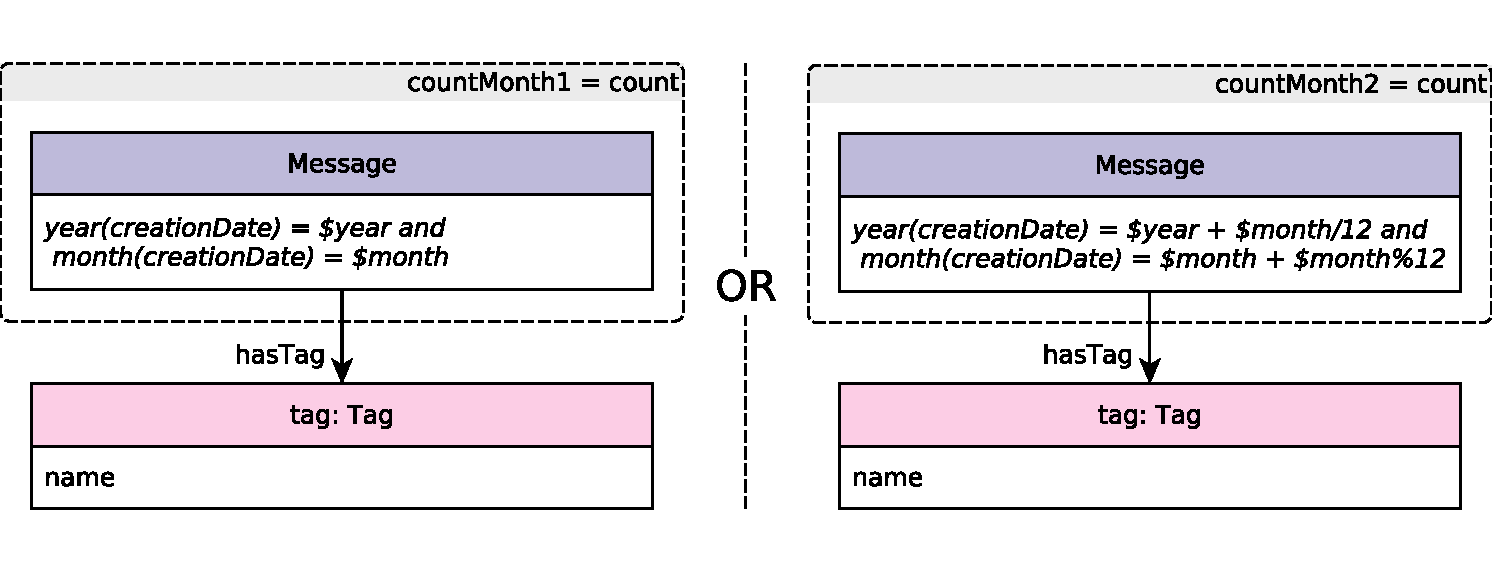
\includegraphics[scale=\patternscale,margin=0cm .2cm]{patterns/bi-read-03}\hfill\vadjust{} \\ \hline
%
	desc. & Given a year and a month, find the Tags that were used in Messages
during the given month of the given year, and the Tags that were used
during the month after the given month of the given year.

For both months, compute the count of Messages that used each of the
Tags.
 \\ \hline
%
	
%
    
        params &
        \innerCardVSpace{\begin{tabularx}{\attributeCardWidth}{|>{\paramNumberCell}c|>{\varNameCell}M|>{\typeCell}m{\typeWidth}|Y|} \hline
        \cellcolor{parameter} \color{white} \footnotesize $\mathsf{1}$ &year& 32-bit Integer &  \\ \hline
        \cellcolor{parameter} \color{white} \footnotesize $\mathsf{2}$ &month& 32-bit Integer &  \\ \hline
        \end{tabularx}}\innerCardVSpace \\ \hline
	
%
	
        result &
        \innerCardVSpace{\begin{tabularx}{\attributeCardWidth}{|>{\resultNumberCell}c|>{\varNameCell}M|>{\typeCell}m{\typeWidth}|>{\resultOriginCell}c|Y|} \hline
        $\mathsf{1}$ & tag.name & String &R&
                 \\ \hline
        $\mathsf{2}$ & countMonth1 & 32-bit Integer &A&
                occurrences of the tag during year-month 1 \\ \hline
        $\mathsf{3}$ & countMonth2 & 32-bit Integer &A&
                occurrences of the tag during year-month 2 \\ \hline
        $\mathsf{4}$ & diff & 32-bit Integer &A&
                difference between occurrences of this Tag in month 1 and month 2 \\ \hline
        \end{tabularx}}\innerCardVSpace \\ \hline
	
%
	sort        &
        \innerCardVSpace{\begin{tabular}{|>{\sortNumberCell}c|>{\varNameCell}l|>{\directionCell}c|} \hline
        $\mathsf{1}$ & diff & $\desc$ \\ \hline
        $\mathsf{2}$ & tag.name & $\asc$ \\ \hline
        \end{tabular}}\innerCardVSpace \\ \hline
	%
	limit & 100 \\ \hline
	%
	CPs &
	\multicolumn{1}{>{\raggedright}l|}{
	    \chokePoint{2.4}, 
	    \chokePoint{3.1}, 
	    \chokePoint{3.2}, 
	    \chokePoint{4.1}, 
	    \chokePoint{4.3}, 
	    \chokePoint{5.3}, 
	    \chokePoint{6.1}
	    } \\ \hline
	%
    %
\end{tabularx}
\queryCardVSpace